\documentclass{standalone}
\usepackage{tikz}
\usepackage{ctex,siunitx}
\setCJKmainfont{Noto Serif CJK SC}
\usepackage{tkz-euclide}
\usepackage{amsmath}
\usetikzlibrary{patterns, calc,3d}
\usetikzlibrary {decorations.pathmorphing,decorations.pathreplacing,decorations.shapes}
\tikzset{label style/.append style={font=\small}}
\begin{document}
\small
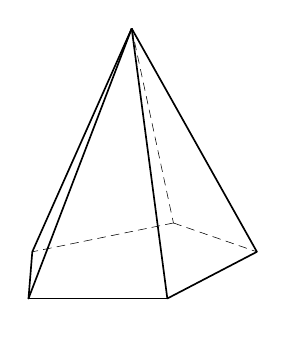
\begin{tikzpicture}[>=latex,scale=1.0,inner sep=1pt]
  \begin{scope}[z={(45:5mm)},canvas is zx plane at y=0]
    \foreach \x[count=\i from 0] in {D,C,B,A,E}
    {\tkzDefPoint(\i*72:1.5){\x}}
    \tkzDefPoints{0/0/O'}
    \tkzDrawSegments[semithick](A,B B,C E,A)
    \tkzDrawSegments[densely dashed](D,E D,C)
    \draw[draw=none](-2.5,0)--(4,0);
  \end{scope}
  \foreach \x in {A,B,C,E}
  {\draw[semithick] (0,3,0)--(\x);}
  \draw[very thin,densely dashed](0,3,0)--(D);
\end{tikzpicture}
\end{document}